% Source: graduate-coursework/Sp26/CSCE763/Course_Assignments/Project/project_proposal.tex
% Description: CA-CFAR detector sliding window architecture (1D cross-section). The cell under test (CUT) is compared against an adaptive threshold derived from surrounding reference cells.

\documentclass[border=4pt]{standalone}
\usepackage{amsmath}
\usepackage{amssymb}
\usepackage{graphicx}
\usepackage{tikz}
\usepackage{xcolor}
\usetikzlibrary{positioning, arrows.meta, calc, fit, backgrounds, decorations.pathreplacing}

\definecolor{USC_Garnet}{HTML}{73000A}
\definecolor{USC_Black10}{HTML}{ECECEC}
\definecolor{USC_Black70}{HTML}{5C5C5C}
\definecolor{USC_Congaree}{HTML}{1F414D}

\begin{document}
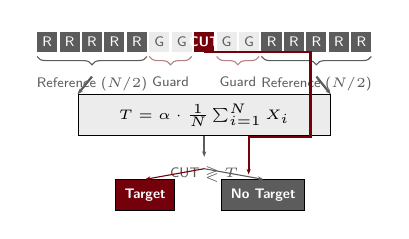
\begin{tikzpicture}[scale=0.75, every node/.style={font=\sffamily\tiny}]
  % Reference cells (left)
  \foreach \i in {0,1,2,3,4} {
    \fill[USC_Black70] (\i*0.38,0) rectangle ++(0.34,0.34);
    \node[white] at (\i*0.38+0.17,0.17) {R};
  }
  % Guard cells (left)
  \foreach \i in {5,6} {
    \fill[USC_Black10] (\i*0.38,0) rectangle ++(0.34,0.34);
    \node[USC_Black70] at (\i*0.38+0.17,0.17) {G};
  }
  % CUT
  \fill[USC_Garnet] (7*0.38,0) rectangle ++(0.34,0.34);
  \node[white, font=\sffamily\tiny\bfseries] at (7*0.38+0.17,0.17) {CUT};
  % Guard cells (right)
  \foreach \i in {8,9} {
    \fill[USC_Black10] (\i*0.38,0) rectangle ++(0.34,0.34);
    \node[USC_Black70] at (\i*0.38+0.17,0.17) {G};
  }
  % Reference cells (right)
  \foreach \i in {10,11,12,13,14} {
    \fill[USC_Black70] (\i*0.38,0) rectangle ++(0.34,0.34);
    \node[white] at (\i*0.38+0.17,0.17) {R};
  }
  % Brace under reference cells
  \draw[decorate, decoration={brace, mirror, amplitude=3pt}, USC_Black70]
    (0,-0.08) -- (4*0.38+0.34,-0.08)
    node[midway, below=4pt, USC_Black70] {Reference ($N/2$)};
  \draw[decorate, decoration={brace, mirror, amplitude=3pt}, USC_Black70]
    (10*0.38,-0.08) -- (14*0.38+0.34,-0.08)
    node[midway, below=4pt, USC_Black70] {Reference ($N/2$)};
  % Brace under guard cells
  \draw[decorate, decoration={brace, mirror, amplitude=3pt}, USC_Garnet!50]
    (5*0.38,-0.08) -- (6*0.38+0.34,-0.08)
    node[midway, below=4pt, USC_Black70] {Guard};
  \draw[decorate, decoration={brace, mirror, amplitude=3pt}, USC_Garnet!50]
    (8*0.38,-0.08) -- (9*0.38+0.34,-0.08)
    node[midway, below=4pt, USC_Black70] {Guard};
  % Arrows from reference cell regions to threshold block
  \coordinate (leftRefMid) at (2*0.38+0.17, -0.08);
  \coordinate (rightRefMid) at (12*0.38+0.17, -0.08);
  % Threshold block
  \node[draw, fill=USC_Black10, minimum height=0.45cm, minimum width=3.2cm,
        font=\sffamily\tiny, anchor=north] (thresh) at (7*0.38+0.17, -0.72)
        {$T = \alpha \cdot \frac{1}{N}\sum_{i=1}^{N} X_i$};
  \draw[-{Stealth[length=2pt]}, thick, USC_Black70] (2*0.38+0.17, -0.42) -- (thresh.north west);
  \draw[-{Stealth[length=2pt]}, thick, USC_Black70] (12*0.38+0.17, -0.42) -- (thresh.north east);
  % Arrow from threshold to comparison point
  \draw[-{Stealth[length=2pt]}, thick, USC_Black70] (thresh.south) -- ++(0,-0.35)
    node[below, font=\sffamily\tiny, USC_Black70] (comp) {CUT $\gtrless$ $T$};
  % Arrow from CUT to comparison point (routed around the right of threshold block)
  \draw[-{Stealth[length=2pt]}, thick, USC_Garnet]
    (7*0.38+0.17, 0) -- ++(1.8,0) -- ++(0,-1.45) -| (comp.east);
  % Decision outputs
  \coordinate (dec) at ($(thresh.south)+(0,-0.55)$);
  \node[draw, fill=USC_Garnet, text=white, minimum height=0.3cm,
        font=\sffamily\tiny\bfseries] (det) at ($(dec)+(-1.0,-0.45)$) {Target};
  \node[draw, fill=USC_Black70, text=white, minimum height=0.3cm,
        font=\sffamily\tiny\bfseries] (nodet) at ($(dec)+(1.0,-0.45)$) {No Target};
  \draw[-{Stealth[length=2pt]}, USC_Garnet] (dec) -- (det.north);
  \draw[-{Stealth[length=2pt]}, USC_Black70] (dec) -- (nodet.north);
\end{tikzpicture}
\end{document}
